\section{Application: Fourier series}

% ----------------------------------------------------------------------
% Legendre 1

\begin{center}
  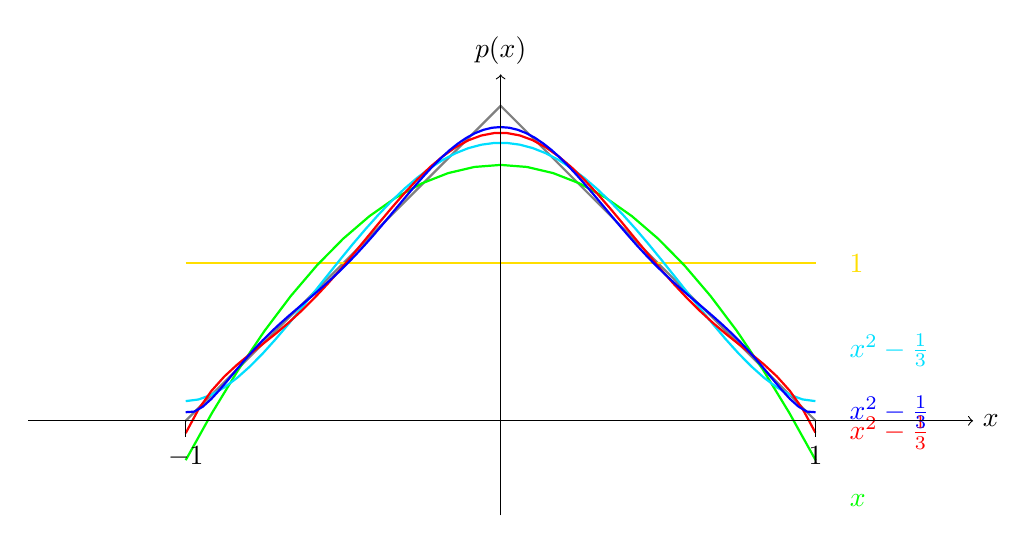
\begin{tikzpicture}[domain=-1:1, scale=4, samples=25]
    \def\fA#1{1}
    \def\fB#1{(#1)}
    \def\fC#1{(abs((#1)^2)-1/3)}
    \def\fD#1{((#1)^3-3/5*(#1))}
    \def\fE#1{(abs((#1)^4)-6/7*abs((#1)^2)+3/35)}
    \def\fF#1{((#1)^5 - 10/9*(#1)^3+5/21*(#1))}
    \def\fG#1{(abs((#1)^6)-15/11*abs((#1)^4)+5/11*abs((#1)^2)-5/231)}
    \def\fH#1{((429*(#1)^7 - 693*(#1)^5 + 315*(#1)^3 - 35*(#1))/429)}
    \def\fI#1{((6435*abs((#1)^8)-12012*abs((#1)^6)+6930*abs((#1)^4)-1260*abs((#1)^2)+35)/6435)}
    \definecolor{my-blue}{rgb}{0,0.87,1.00}
    \definecolor{my-yellow}{rgb}{1.00,0.87,0.00}
    \draw[thick,color=gray] (-1,0) -- (0,1) -- (1,0);
    \draw[thick,color=my-yellow] plot (\x,0.5*\fA{\x}) node[right=2ex] {$1$};
    \draw[thick,color=green] plot (\x,{0.5*\fA{\x} - 0.9375*\fC{\x}}) node[below right=2ex] {$x$};
    \draw[thick,color=my-blue,samples=50] plot (\x,{0.5*\fA{\x} - 0.9375*\fC{\x} + 0.8203125*\fE{\x}}) node[above right=2ex] {$x^2-\frac{1}{3}$};
    \draw[thick,color=red,samples=50] plot (\x,{0.5*\fA{\x} - 0.9375*\fC{\x} + 0.8203125*\fE{\x} -1.46630859375*\fG{\x}}) node[right=2ex] {$x^2-\frac{1}{3}$};
    \draw[thick,color=blue,samples=75] plot (\x,{0.5*\fA{\x} - 0.9375*\fC{\x} + 0.8203125*\fE{\x} -1.46630859375*\fG{\x}+3.338470458984375*\fI{\x}}) node[right=2ex] {$x^2-\frac{1}{3}$};
    \draw[->] (-1.5,0) -- (1.5,0) node[right] {$x$};
    \draw[->] (0,-0.3) -- (0,1.1) node[above] {$p(x)$};
    \draw (1,0) -- (1,-0.05) node[below] {$1$};
    \draw (-1,0) -- (-1,-0.05) node[below] {$-1$};
  \end{tikzpicture}
\end{center}

% ----------------------------------------------------------------------
% Legendre 2

\begin{center}
  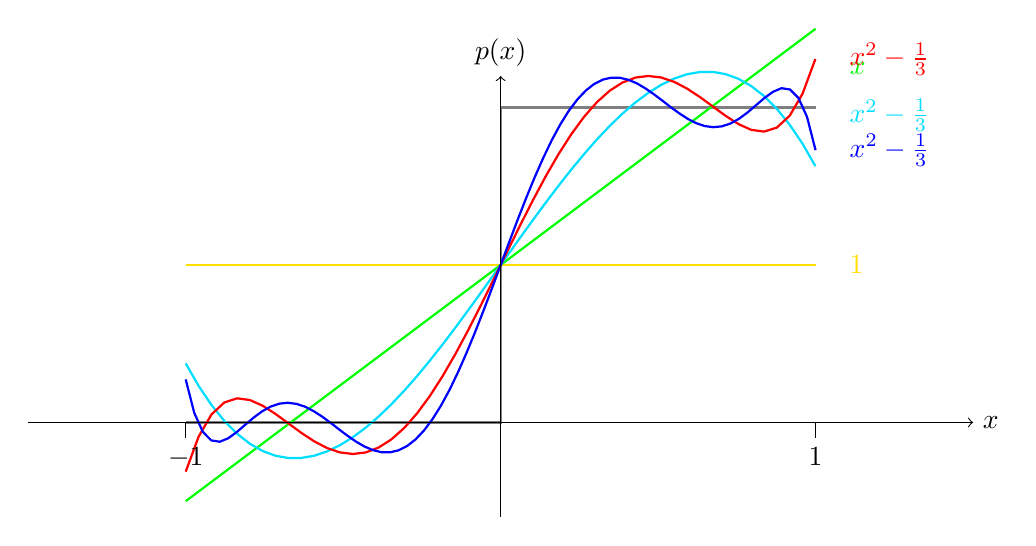
\begin{tikzpicture}[domain=-1:1, scale=4, samples=25]
    \def\fA#1{1}
    \def\fB#1{(#1)}
    \def\fC#1{(abs((#1)^2)-1/3)}
    \def\fD#1{((#1)^3-3/5*(#1))}
    \def\fE#1{(abs((#1)^4)-6/7*abs((#1)^2)+3/35)}
    \def\fF#1{((#1)^5 - 10/9*(#1)^3+5/21*(#1))}
    \def\fG#1{(abs((#1)^6)-15/11*abs((#1)^4)+5/11*abs((#1)^2)-5/231)}
    \def\fH#1{((429*(#1)^7 - 693*(#1)^5 + 315*(#1)^3 - 35*(#1))/429)}
    \def\fI#1{((6435*abs((#1)^8)-12012*abs((#1)^6)+6930*abs((#1)^4)-1260*abs((#1)^2)+35)/6435)}
    \definecolor{my-blue}{rgb}{0,0.87,1.00}
    \definecolor{my-yellow}{rgb}{1.00,0.87,0.00}
    \draw[thick,color=gray] (-1,0) -- (0,0) -- (0,1) -- (1,1);
    \draw[thick,color=my-yellow] plot (\x,0.5*\fA{\x}) node[right=2ex] {$1$};
    \draw[thick,color=green]     plot (\x,{0.5*\fA{\x} + 0.75*\fB{\x}}) node[below right=2ex] {$x$};
    \draw[thick,color=my-blue,samples=50]   plot (\x,{0.5*\fA{\x} + 0.75*\fB{\x} - 1.09375*\fD{\x}}) node[above right=2ex] {$x^2-\frac{1}{3}$};
    \draw[thick,color=red,samples=50]       plot (\x,{0.5*\fA{\x} + 0.75*\fB{\x} - 1.09375*\fD{\x} + 2.70703125*\fF{\x}}) node[right=2ex] {$x^2-\frac{1}{3}$};
    \draw[thick,color=blue,samples=75]      plot (\x,{0.5*\fA{\x} + 0.75*\fB{\x} - 1.09375*\fD{\x} + 2.70703125*\fF{\x} - 7.855224609375*\fH{\x}}) node[right=2ex] {$x^2-\frac{1}{3}$};
    \draw[->] (-1.5,0) -- (1.5,0) node[right] {$x$};
    \draw[->] (0,-0.3) -- (0,1.1) node[above] {$p(x)$};
    \draw (1,0) -- (1,-0.05) node[below] {$1$};
    \draw (-1,0) -- (-1,-0.05) node[below] {$-1$};
  \end{tikzpicture}
\end{center}

% ----------------------------------------------------------------------
% Legendre 3

\begin{center}
  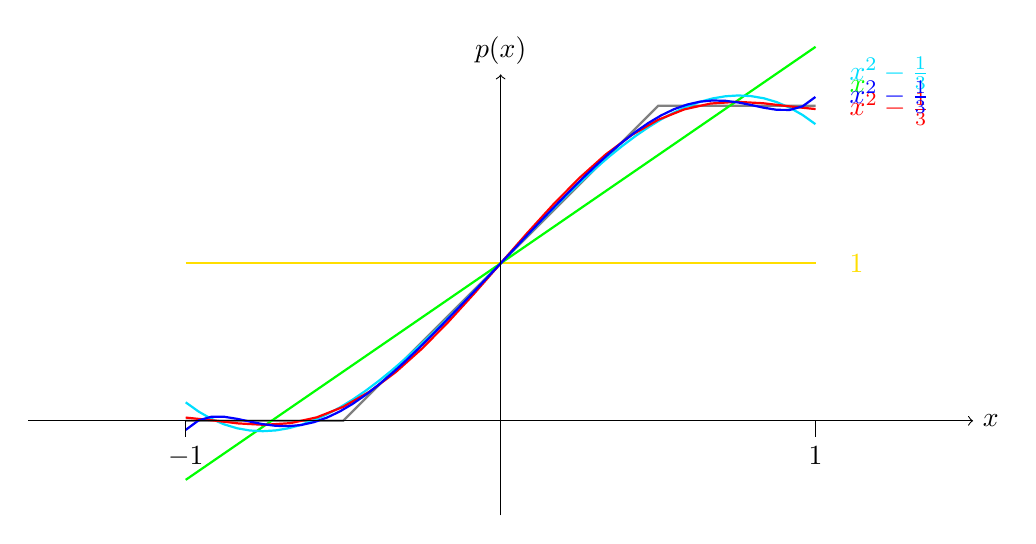
\begin{tikzpicture}[domain=-1:1, scale=4, samples=25]
    \def\fA#1{1}
    \def\fB#1{(#1)}
    \def\fC#1{(abs((#1)^2)-1/3)}
    \def\fD#1{((#1)^3-3/5*(#1))}
    \def\fE#1{(abs((#1)^4)-6/7*abs((#1)^2)+3/35)}
    \def\fF#1{((#1)^5 - 10/9*(#1)^3+5/21*(#1))}
    \def\fG#1{(abs((#1)^6)-15/11*abs((#1)^4)+5/11*abs((#1)^2)-5/231)}
    \def\fH#1{((429*(#1)^7 - 693*(#1)^5 + 315*(#1)^3 - 35*(#1))/429)}
    \def\fI#1{((6435*abs((#1)^8)-12012*abs((#1)^6)+6930*abs((#1)^4)-1260*abs((#1)^2)+35)/6435)}
    \definecolor{my-blue}{rgb}{0,0.87,1.00}
    \definecolor{my-yellow}{rgb}{1.00,0.87,0.00}
    \draw[thick,color=gray] (-1,0) -- (-0.5,0) -- (0.5,1) -- (1,1);
    \draw[thick,color=my-yellow] plot (\x,0.5*\fA{\x}) node[right=2ex] {$1$};
    \draw[thick,color=green]     plot (\x,{0.5*\fA{\x} + 0.6875*\fB{\x}}) node[below right=2ex] {$x$};
    \draw[thick,color=my-blue,samples=50]   plot (\x,{0.5*\fA{\x} + 0.6875*\fB{\x} - 0.615234375*\fD{\x}}) node[above right=2ex] {$x^2-\frac{1}{3}$};
    \draw[thick,color=red]       plot (\x,{0.5*\fA{\x} + 0.6875*\fB{\x} - 0.615234375*\fD{\x} + 0.38067626953125*\fF{\x}}) node[right=2ex] {$x^2-\frac{1}{3}$};
    \draw[thick,color=blue,samples=50]      plot (\x,{0.5*\fA{\x} + 0.6875*\fB{\x} - 0.615234375*\fD{\x} + 0.38067626953125*\fF{\x} + 1.0494089126587303*\fH{\x}}) node[right=2ex] {$x^2-\frac{1}{3}$};
    \draw[->] (-1.5,0) -- (1.5,0) node[right] {$x$};
    \draw[->] (0,-0.3) -- (0,1.1) node[above] {$p(x)$};
    \draw (1,0) -- (1,-0.05) node[below] {$1$};
    \draw (-1,0) -- (-1,-0.05) node[below] {$-1$};
  \end{tikzpicture}
\end{center}

% ----------------------------------------------------------------------
% Fourier 1

\begin{center}
  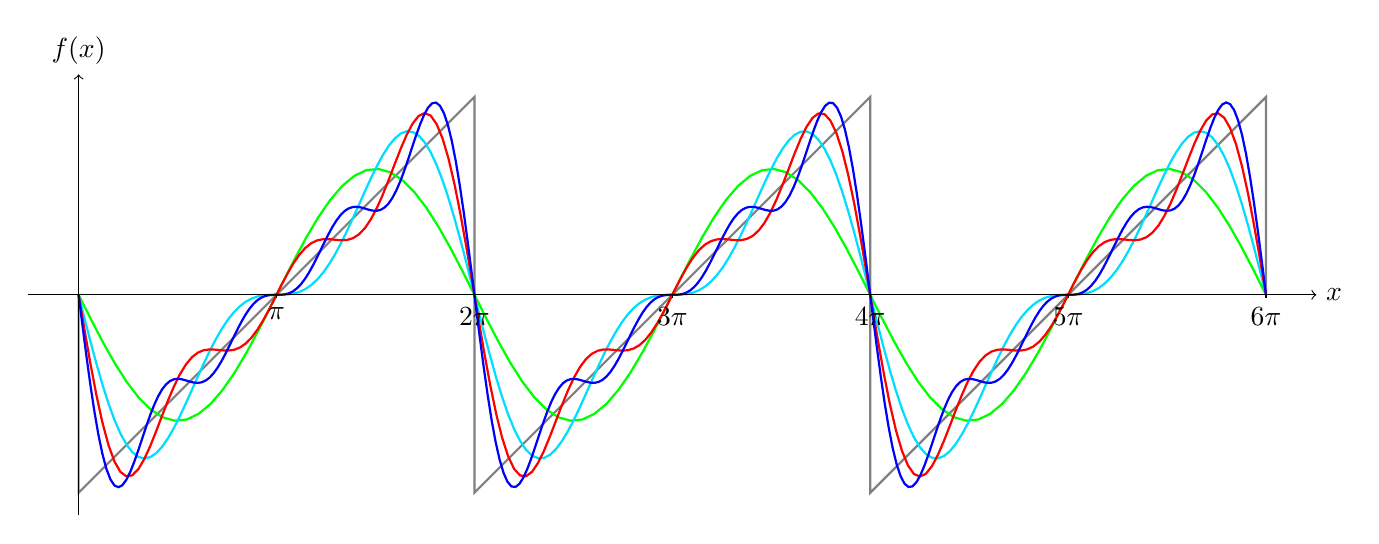
\begin{tikzpicture}[domain=0:6*pi, scale=0.8, samples=100]
    \def\fA#1{1}
    \def\fB#1{(sin((#1)/pi*180)}
    \def\fC#1{(cos((#1)/pi*180))}
    \def\fD#1{(sin(2*(#1)/pi*180))}
    \def\fE#1{(cos(2*(#1)/pi*180))}
    \def\fF#1{(sin(3*(#1)/pi*180))}
    \def\fG#1{(cos(3*(#1)/pi*180))}
    \def\fH#1{(sin(4*(#1)/pi*180))}
    \def\fI#1{(cos(4*(#1)/pi*180))}
    \definecolor{my-blue}{rgb}{0,0.87,1.00}
    \definecolor{my-yellow}{rgb}{1.00,0.87,0.00}
    \draw[thick,color=gray] (0,0) -- (0,-pi) -- (2*pi,pi) -- (2*pi,-pi) --
    (4*pi,pi) -- (4*pi,-pi) -- (6*pi, pi) -- (6*pi, 0);
    \draw[thick,color=green]   plot (\x,{((-2)*\fB{\x})}) node[below right=2ex] {};
    \draw[thick,color=my-blue,samples=200] plot (\x,{((-2)*\fB{\x})+((-1)*\fD{\x})}) node[above right=2ex] {};
    \draw[thick,color=red,samples=200]     plot (\x,{((-2)*\fB{\x})+((-1)*\fD{\x})+((-2/3)*\fF{\x})}) node[right=2ex] {};
    \draw[thick,color=blue,samples=300]    plot (\x,{((-2)*\fB{\x})+((-1)*\fD{\x})+((-2/3)*\fF{\x})+((-1/2)*\fH{\x})}) node[right=2ex] {};
    \draw[->] (-0.8,0) -- (6*pi+0.8,0) node[right] {$x$};
    \draw[->] (0,-3.5) -- (0,3.5) node[above] {$f(x)$};
    \draw (pi,0) -- (pi,-0.05) node[below] {$\pi$};
    \draw (2*pi,0) -- (2*pi,-0.05) node[below] {$2\pi$};
    \draw (3*pi,0) -- (3*pi,-0.05) node[below] {$3\pi$};
    \draw (4*pi,0) -- (4*pi,-0.05) node[below] {$4\pi$};
    \draw (5*pi,0) -- (5*pi,-0.05) node[below] {$5\pi$};
    \draw (6*pi,0) -- (6*pi,-0.05) node[below] {$6\pi$};
  \end{tikzpicture}
\end{center}

\begin{center}
  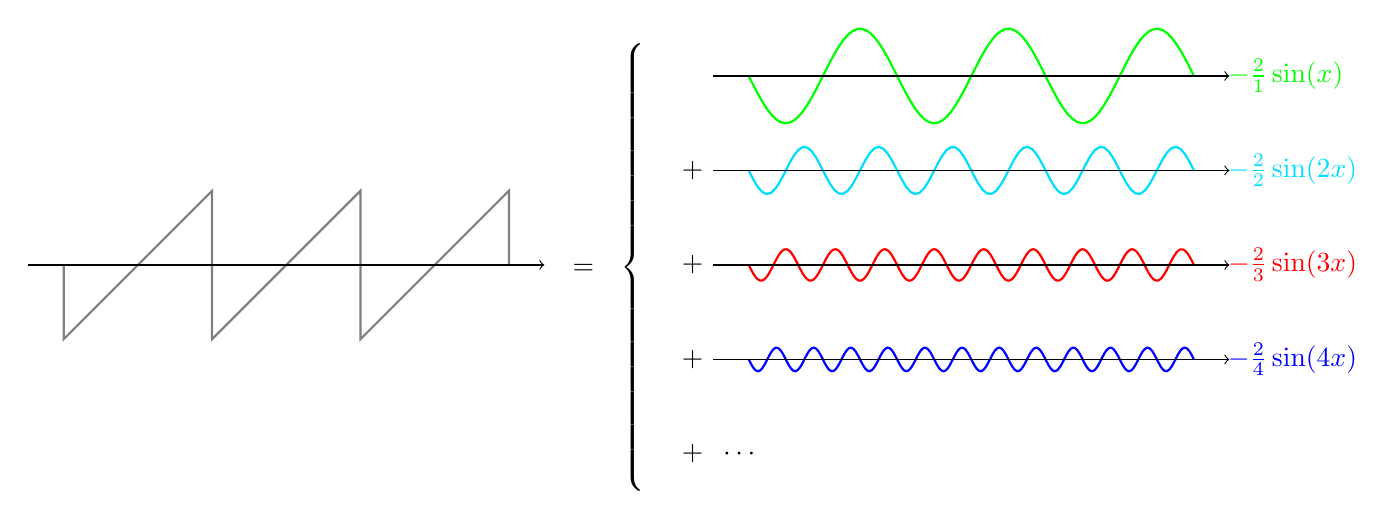
\begin{tikzpicture}[domain=0:6*pi, scale=0.3, samples=100]
    \def\fA#1{1}
    \def\fB#1{(sin((#1)/pi*180)}
    \def\fC#1{(cos((#1)/pi*180))}
    \def\fD#1{(sin(2*(#1)/pi*180))}
    \def\fE#1{(cos(2*(#1)/pi*180))}
    \def\fF#1{(sin(3*(#1)/pi*180))}
    \def\fG#1{(cos(3*(#1)/pi*180))}
    \def\fH#1{(sin(4*(#1)/pi*180))}
    \def\fI#1{(cos(4*(#1)/pi*180))}
    \definecolor{my-blue}{rgb}{0,0.87,1.00}
    \definecolor{my-yellow}{rgb}{1.00,0.87,0.00}
    \begin{scope}[yshift=-12cm,xshift=-29cm]
      \draw[thick,color=gray] (0,0) -- (0,-pi) -- (2*pi,pi) -- (2*pi,-pi) --
      (4*pi,pi) -- (4*pi,-pi) -- (6*pi, pi) -- (6*pi, 0);
      \draw[->] (-1.5,0) -- (6*pi+1.5,0)
      node[right]{$~~=~~\left\{\rule{0mm}{3cm}\right.$};
    \end{scope}
    \begin{scope}[yshift=-4cm]
      \draw[thick,color=green]   plot (\x,{((-2)*\fB{\x})}) node[right=2ex] {$-\frac{2}{1}\sin(x)$};
      \draw[->] (-1.5,0) -- (6*pi+1.5,0);
    \end{scope}
    \begin{scope}[yshift=-8cm]
      \draw[thick,color=my-blue] plot (\x,{((-1)*\fD{\x})}) node[right=2ex] {$-\frac{2}{2}\sin(2x)$};
      \draw[->] (-1.5,0) node[left]{$+$} -- (6*pi+1.5,0);
    \end{scope}
    \begin{scope}[yshift=-12cm]
      \draw[thick,color=red,samples=200]     plot (\x,{((-2/3)*\fF{\x})}) node[right=2ex] {$-\frac{2}{3}\sin(3x)$};
      \draw[->] (-1.5,0) node[left]{$+$} -- (6*pi+1.5,0);
    \end{scope}
    \begin{scope}[yshift=-16cm]
      \draw[thick,color=blue,samples=200]    plot (\x,{((-1/2)*\fH{\x})}) node[right=2ex] {$-\frac{2}{4}\sin(4x)$};
      \draw[->] (-1.5,0) node[left]{$+$} -- (6*pi+1.5,0);
    \end{scope}
    \begin{scope}[yshift=-20cm]
      \path (-1.5,0) node[left]{$+$} node[right]{$\cdots$};
    \end{scope}
  \end{tikzpicture}
\end{center}

% ----------------------------------------------------------------------
% Fourier 2

\begin{center}
  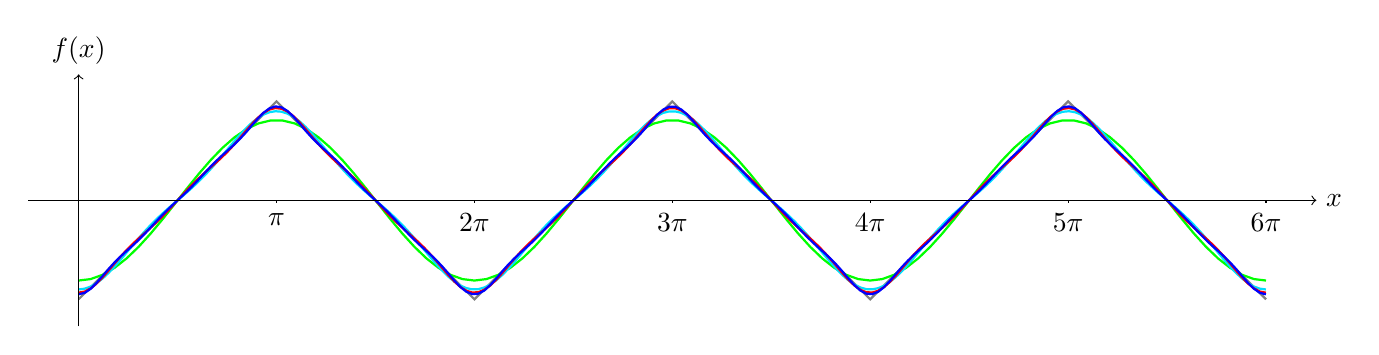
\begin{tikzpicture}[domain=0:6*pi, scale=0.8, samples=100]
    \def\fC#1{(cos((#1)/pi*180))}
    \def\fG#1{(cos(3*(#1)/pi*180))}
    \def\fK#1{(cos(5*(#1)/pi*180))}
    \def\fO#1{(cos(7*(#1)/pi*180))}
    \definecolor{my-blue}{rgb}{0,0.87,1.00}
    \definecolor{my-yellow}{rgb}{1.00,0.87,0.00}
    \draw[thick,color=gray] (0,-pi/2) -- (pi,pi/2) -- (2*pi,-pi/2) -- (3*pi,pi/2) --
    (4*pi,-pi/2) -- (5*pi,pi/2) -- (6*pi, -pi/2);
    \draw[thick,color=green]   plot (\x,{((-1.2732395447351623)*\fC{\x})}) node[below right=2ex] {};
    \draw[thick,color=my-blue,samples=200] plot (\x,{((-1.2732395447351623)*\fC{\x})+((-0.14147106052612904)*\fG{\x})}) node[above right=2ex] {};
    \draw[thick,color=red,samples=200]     plot (\x,{((-1.2732395447351623)*\fC{\x})+((-0.14147106052612904)*\fG{\x})+((-0.05092958178940641)*\fK{\x})}) node[above right=2ex] {};
    \draw[thick,color=blue,samples=200]    plot (\x,{((-1.2732395447351623)*\fC{\x})+((-0.14147106052612904)*\fG{\x})+((-0.05092958178940641)*\fK{\x})+((-0.025984480504798825)*\fO{\x})}) node[above right=2ex] {};
    \draw[->] (-0.8,0) -- (6*pi+0.8,0) node[right] {$x$};
    \draw[->] (0,-2) -- (0,2) node[above] {$f(x)$};
    \draw (pi,0) -- (pi,-0.05) node[below] {$\pi$};
    \draw (2*pi,0) -- (2*pi,-0.05) node[below] {$2\pi$};
    \draw (3*pi,0) -- (3*pi,-0.05) node[below] {$3\pi$};
    \draw (4*pi,0) -- (4*pi,-0.05) node[below] {$4\pi$};
    \draw (5*pi,0) -- (5*pi,-0.05) node[below] {$5\pi$};
    \draw (6*pi,0) -- (6*pi,-0.05) node[below] {$6\pi$};
  \end{tikzpicture}
\end{center}

\begin{center}
  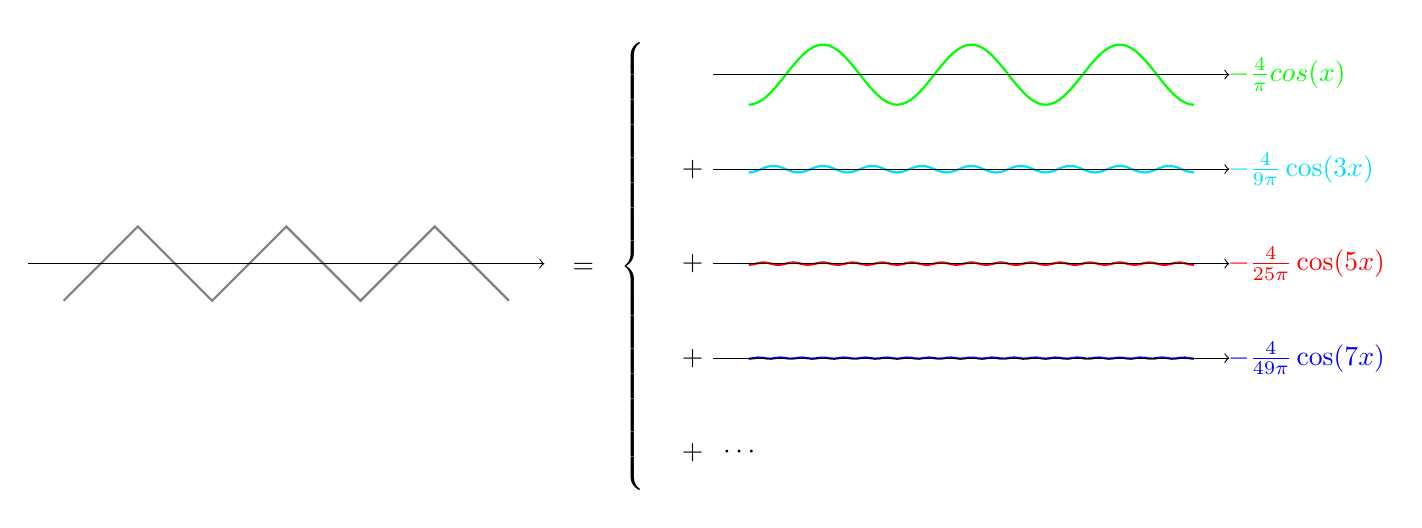
\begin{tikzpicture}[domain=0:6*pi, scale=0.3, samples=100]
    \def\fC#1{(cos((#1)/pi*180))}
    \def\fG#1{(cos(3*(#1)/pi*180))}
    \def\fK#1{(cos(5*(#1)/pi*180))}
    \def\fO#1{(cos(7*(#1)/pi*180))}
    \definecolor{my-blue}{rgb}{0,0.87,1.00}
    \definecolor{my-yellow}{rgb}{1.00,0.87,0.00}
    \begin{scope}[yshift=-12cm,xshift=-29cm]
      \draw[thick,color=gray] (0,-pi/2) -- (pi,pi/2) -- (2*pi,-pi/2) -- (3*pi,pi/2) --
      (4*pi,-pi/2) -- (5*pi,pi/2) -- (6*pi, -pi/2);
      \draw[->] (-1.5,0) -- (6*pi+1.5,0)
      node[right]{$~~=~~\left\{\rule{0mm}{3cm}\right.$};
    \end{scope}
    \begin{scope}[yshift=-4cm]
      \draw[thick,color=green]   plot (\x,{((-1.2732395447351623)*\fC{\x})}) (6*pi,0) node[right=2ex] {$-\frac{4}{\pi}cos(x)$};
      \draw[->] (-1.5,0) -- (6*pi+1.5,0);
    \end{scope}
    \begin{scope}[yshift=-8cm]
      \draw[thick,color=my-blue] plot (\x,{((-0.14147106052612904)*\fG{\x})}) (6*pi,0) node[right=2ex] {$-\frac{4}{9\pi}\cos(3x)$};
      \draw[->] (-1.5,0) node[left]{$+$} -- (6*pi+1.5,0);
    \end{scope}
    \begin{scope}[yshift=-12cm]
      \draw[thick,color=red]     plot (\x,{((-0.05092958178940641)*\fK{\x})}) (6*pi,0) node[right=2ex] {$-\frac{4}{25\pi}\cos(5x)$};
      \draw[->] (-1.5,0) node[left]{$+$} -- (6*pi+1.5,0);
    \end{scope}
    \begin{scope}[yshift=-16cm]
      \draw[thick,color=blue]    plot (\x,{((-0.025984480504798825)*\fO{\x})}) (6*pi,0) node[right=2ex] {$-\frac{4}{49\pi}\cos(7x)$};
      \draw[->] (-1.5,0) node[left]{$+$} -- (6*pi+1.5,0);
    \end{scope}
    \begin{scope}[yshift=-20cm]
      \path (-1.5,0) node[left]{$+$} node[right]{$\cdots$};
    \end{scope}
  \end{tikzpicture}
\end{center}

% ----------------------------------------------------------------------
% Fourier 3

\begin{center}
  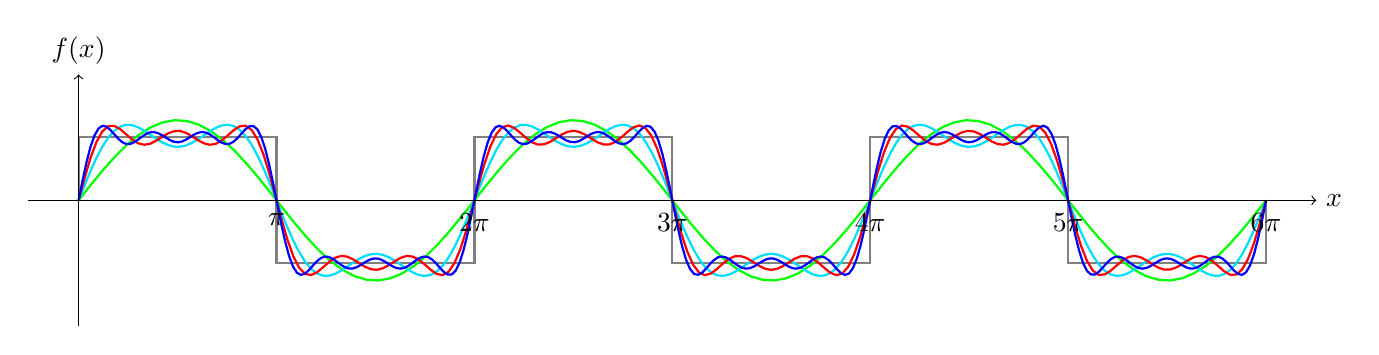
\begin{tikzpicture}[domain=0:6*pi, scale=0.8, samples=100]
    \def\fB#1{(sin((#1)/pi*180))}
    \def\fF#1{(sin(3*(#1)/pi*180))}
    \def\fJ#1{(sin(5*(#1)/pi*180))}
    \def\fN#1{(sin(7*(#1)/pi*180))}
    \definecolor{my-blue}{rgb}{0,0.87,1.00}
    \definecolor{my-yellow}{rgb}{1.00,0.87,0.00}
    \draw[thick,color=gray] (0,0) -- (0,1) -- (pi,1) -- (pi,-1) --
    (2*pi,-1) -- (2*pi,1) --
    (3*pi,1) -- (3*pi,-1) --
    (4*pi,-1) -- (4*pi,1) --
    (5*pi,1) -- (5*pi,-1) --
    (6*pi,-1) -- (6*pi,0);
    \draw[thick,color=green]   plot (\x,{((1.2732395447351623)*\fB{\x})}) node[below right=2ex] {};
    \draw[thick,color=my-blue,samples=200] plot (\x,{((1.2732395447351623)*\fB{\x})+((0.4244131815783881)*\fF{\x})}) node[above right=2ex] {};
    \draw[thick,color=red,samples=200]     plot (\x,{((1.2732395447351623)*\fB{\x})+((0.4244131815783881)*\fF{\x})+((0.25464790894703326)*\fJ{\x})}) node[above right=2ex] {};
    \draw[thick,color=blue,samples=300]    plot (\x,{((1.2732395447351623)*\fB{\x})+((0.4244131815783881)*\fF{\x})+((0.25464790894703326)*\fJ{\x})+((0.18189136353359486)*\fN{\x})}) node[above right=2ex] {};
    \draw[->] (-0.8,0) -- (6*pi+0.8,0) node[right] {$x$};
    \draw[->] (0,-2) -- (0,2) node[above] {$f(x)$};
    \draw (pi,0) -- (pi,-0.05) node[below] {$\pi$};
    \draw (2*pi,0) -- (2*pi,-0.05) node[below] {$2\pi$};
    \draw (3*pi,0) -- (3*pi,-0.05) node[below] {$3\pi$};
    \draw (4*pi,0) -- (4*pi,-0.05) node[below] {$4\pi$};
    \draw (5*pi,0) -- (5*pi,-0.05) node[below] {$5\pi$};
    \draw (6*pi,0) -- (6*pi,-0.05) node[below] {$6\pi$};
  \end{tikzpicture}
\end{center}

\begin{center}
  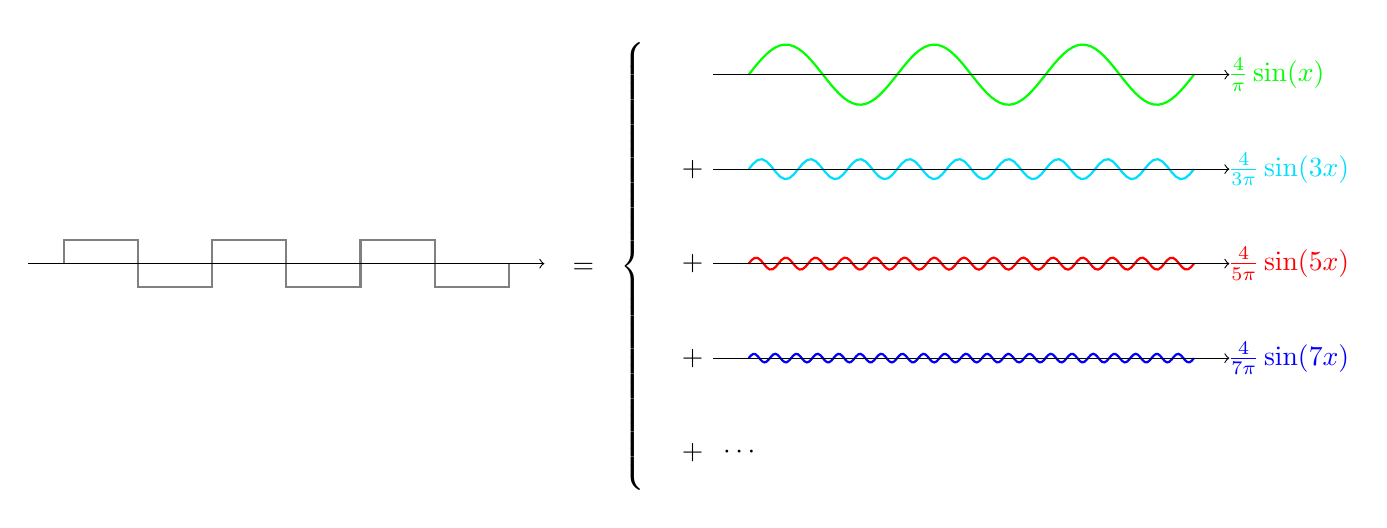
\begin{tikzpicture}[domain=0:6*pi, scale=0.3, samples=100]
    \def\fB#1{(sin((#1)/pi*180))}
    \def\fF#1{(sin(3*(#1)/pi*180))}
    \def\fJ#1{(sin(5*(#1)/pi*180))}
    \def\fN#1{(sin(7*(#1)/pi*180))}
    \definecolor{my-blue}{rgb}{0,0.87,1.00}
    \definecolor{my-yellow}{rgb}{1.00,0.87,0.00}
    \begin{scope}[yshift=-12cm,xshift=-29cm]
      \draw[thick,color=gray] (0,0) -- (0,1) -- (pi,1) -- (pi,-1) --
      (2*pi,-1) -- (2*pi,1) --
      (3*pi,1) -- (3*pi,-1) --
      (4*pi,-1) -- (4*pi,1) --
      (5*pi,1) -- (5*pi,-1) --
      (6*pi,-1) -- (6*pi,0);
      \draw[->] (-1.5,0) -- (6*pi+1.5,0)
      node[right]{$~~=~~\left\{\rule{0mm}{3cm}\right.$};
    \end{scope}
    \begin{scope}[yshift=-4cm]
      \draw[thick,color=green]   plot (\x,{((1.2732395447351623)*\fB{\x})}) node[right=2ex] {$\frac{4}{\pi}\sin(x)$};
      \draw[->] (-1.5,0) -- (6*pi+1.5,0);
    \end{scope}
    \begin{scope}[yshift=-8cm]
      \draw[thick,color=my-blue] plot (\x,{((0.4244131815783881)*\fF{\x})}) node[right=2ex] {$\frac{4}{3\pi}\sin(3x)$};
      \draw[->] (-1.5,0) node[left]{$+$} -- (6*pi+1.5,0);
    \end{scope}
    \begin{scope}[yshift=-12cm]
      \draw[thick,color=red,samples=150]     plot (\x,{((0.25464790894703326)*\fJ{\x})}) node[right=2ex] {$\frac{4}{5\pi}\sin(5x)$};
      \draw[->] (-1.5,0) node[left]{$+$} -- (6*pi+1.5,0);
    \end{scope}
    \begin{scope}[yshift=-16cm]
      \draw[thick,color=blue,samples=200]    plot (\x,{((0.18189136353359486)*\fN{\x})}) node[right=2ex] {$\frac{4}{7\pi}\sin(7x)$};
      \draw[->] (-1.5,0) node[left]{$+$} -- (6*pi+1.5,0);
    \end{scope}
    \begin{scope}[yshift=-20cm]
      \path (-1.5,0) node[left]{$+$} node[right]{$\cdots$};
    \end{scope}
  \end{tikzpicture}
\end{center}
